不同编程语言的执行模型也不同,最常见的便是解释语言和编译语言。编译器将源代码翻译成机器代码,计算机可以在没有中间系统支持的环境下运行。另外,解释性语言代码需要支持系统、解释器和虚拟环境才能工作。 \par
C++是编译语言,所以会比解释型程序运行得更快。但C++程序需要针对每个平台进行编译,但解释型程序可以跨平台运行。 \par
我们将讨论程序构建的细节,从源代码阶段开始——由编译器完成——到可执行文件(编译器的输出)结束。还会去了解,为什么为一个平台构建的程序不能在另一个平台上运行。 \par
本章将讨论以下主题: \par

\begin{itemize}
	\item 介绍C++20。
	\item C++预处理的细节。
	\item 源代码的(底层)编译。
	\item 了解连接器及其功能。
	\item 加载和运行可执行文件的过程。
\end{itemize}

\noindent\textbf{}\ \par
\textbf{技术要求} \\
g++编译器需要添加编译选项 \texttt{-std=c++2a} 来编译本章的代码。可以从这里获取本章的源码文件:https:/​/github.​com/PacktPublishing/Expert-CPP \par

\noindent\textbf{}\ \par
\textbf{介绍C++20} \\
C++经过多年的发展,目前发展到C++ 20。自C++ 11以来,C++标准已经对语言的特性集进行了极大地扩展。现在,让我们来看看C++ 20标准中哪些值得关注的特性。 \par

\noindent\textbf{}\ \par
\textbf{概念(Concepts):}\ \par
概念是C++ 20的主要特性之一,它为类型提供了一组需求。概念的基本思想是模板参数的编译时进行验证,例如:要指定模板实参必须有默认构造函数,可以使用\textbf{default\underline{ }constructible}概念,方法如下: \par
\noindent\textbf{}\ \par

	%template <\textbf{default\underline{ }constructible} T> \par
	%void make\underline{ }T() { return T(); } \par
	
\begin{lstlisting}[caption={}]
template <default_constructible T>
void make_T() { return T(); }
\end{lstlisting}
	
\noindent\textbf{}\ \par
上面的代码中,我们忽略了typename关键字,设置一个概念来描述模板函数的形参T。\par

可以说概念是描述其他类型的类型——可称为元类型。允许在编译时验证模板参数,以及基于类型属性的函数调用。我们将在第3章和第4章中详细讨论这些概念。 \par

\noindent\textbf{}\ \par
\textbf{协程(Coroutines):}\ \par
协程是能够在执行点停止,并在稍后恢复的特殊函数。协程用以下关键字进行扩展:\par

\begin{enumerate}
	\item \texttt{co\underline{ }await} 暂停协程的执行。
	\item \texttt{co\underline{ }yield} 暂停协程的执行,同时返回一个值。
	\item \texttt{co\underline{ }return} 类似于return,完成协程时返回一个值。举个栗子:
\end{enumerate}

%	generator<int> step\underline{ }by\underline{ }step(int n = 0) \{ \par
%		\quad while (true) \{ \par
%			\quad \quad \textbf{co\underline{ }yield} n++; \par
%		\quad \} \par
%	\} \par

\begin{lstlisting}[caption={}]
generator<int> step_by_step(int n = 0) {
	while (true) {
		co_yield n++;
	}
}
\end{lstlisting}

\noindent\textbf{}\ \par
协程与promise对象相关联,promise可以存储协程的状态并发出警报。我们将在第8章中更深入地研究协程。 \par
	
\noindent\textbf{}\ \par
\textbf{范围(Ranges):}\ \par
范围库提供了一种处理元素范围的新方法。要使用它们,首先要包含<ranges>头文件。来看一个例子,范围是一个有开始和结束的元素vector,提供了一个begin迭代器和一个end哨兵:\par

\begin{lstlisting}[caption={}]
import <vector>
int main()
{
	std::vector<int> elements{0, 1, 2, 3, 4, 5, 6};
}
\end{lstlisting}

带有范围适配器(\texttt{|}操作符)的范围支持处理一系列元素的功能。看下代码: \par

\begin{lstlisting}[caption={}]
import <vector>
import <ranges>
int main()
{
	std::vector<int> elements{0, 1, 2, 3, 4, 5, 6};
	for (int current : elements | ranges::view::filter([](int e) { return
		e % 2 == 0; }))
	{
		std::cout << current << " ";
	}
}
\end{lstlisting}

前面的代码中,使用\texttt{ranges::view::filter()}过滤偶数。请注意\texttt{|}可以在不同的vector间使用。我们将在第7章中讨论范围及其强大的特性。 \par

\noindent\textbf{}\ \par
\textbf{更多C++20的特性}\ \par
C++ 20是一个大版本,它包含了许多更加复杂和灵活的特性。概念、范围和协程是本书讨论的众多特性中部分。 \par
最受期待的特性(之一)是模块,它提供了声明模块,以及在这些模块中导出类型和值的能力。可以将模块视为带有包含保护头文件,也就是头文件的改进版本。本章将介绍C++20中模块的特性。 \par
除了C++ 20中添加的一些特性外,我们还将在本书中讨论其他一些特性: \par

\begin{itemize}
	\item 超级操作符: \texttt{operator<=>()}。 现在可以利用\texttt{<=>()}来控制操作符重载的冗长程度。
	\item \texttt{constexpr}在这门语言中越来越常见。C++ 20现在添加了\texttt{consteval}函数、\texttt{constexpr std::vector}和\texttt{std::string}等类型。
	\item 数学常量,如\texttt{std::number::pi}和\texttt{std::number::log2e}。
	\item 线程库的更新,包括停止令牌和加入线程。
	\item 概念迭代器。
	\item 仅移动视图和其他功能。
\end{itemize}

为了更好地理解一些新特性并深入到该语言的本质,我们将从以前的版本开始介绍该语言的核心。这将有助于我们找到新特性相对于旧特性的更好用法,也将有助于支持历史遗留的C++代码。现在让我们从理解C++应用程序的构建开始。 \par

\noindent\textbf{}\ \par
\textbf{Building and running programs}\ \par
You can use any text editor to write code, because, ultimately, code is just text. To write code, you are free to choose between simple text editors such as Vim, or an advanced integrated development environment (IDE) such as MS Visual Studio. The only difference between a love letter and source code is that the latter might be interpreted by a special program called a compiler (while the love letter cannot be compiled into a program, it might give you butterflies in your stomach). \par
To mark the difference between a plain text file and source code, a special file extension is used. C++ operates with the  .cpp and  .h extensions (you may also occasionally encounter .cxx and  .hpp as well). Before getting into the details, think of the compiler as a tool that translates the source code into a runnable program, known as an executable file or just an executable. The process of making an executable from the source code is called compilation. Compiling a C++ program is a sequence of complex tasks that results in machine code generation. Machine code is the native language of the computer—that's why it's called machine code. \par
Typically, a C++ compiler parses and analyzes the source code, then generates intermediate code, optimizes it, and finally, generates machine code in a file called an object file. You may have already encountered object files; they have individual extensions –  .o in Linux and  .obj in Windows. The created object file contains more than just machine code that can be run by the computer. Compilation usually involves several source files, and compiling each source file produces a separate object file. These object files are then linked together by a tool called the linker to form a single executable file. The linker uses additional information stored in object files to link them properly (linking will be discussed later in this chapter). \par
The following diagram depicts the program-building phases: \par

\begin{center}
	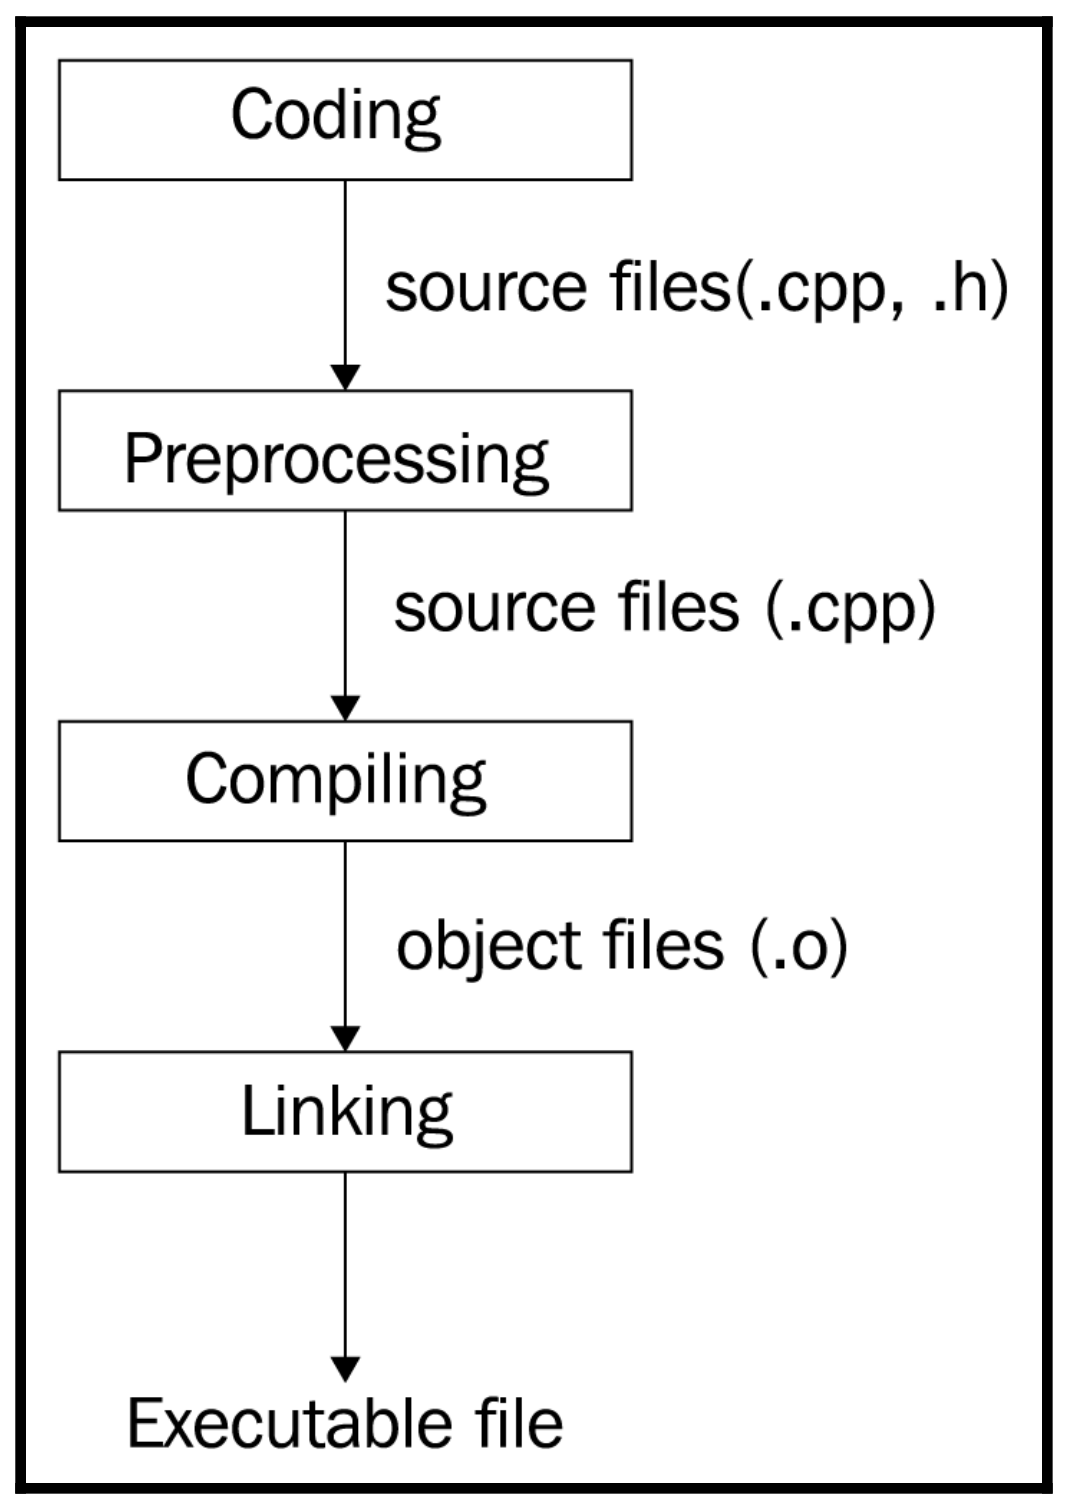
\includegraphics[width=0.3\textwidth]{content/Section-1/Chapter-1/1}
\end{center}

The C++ application-building process consists of three major steps: preprocessing, compiling, and linking. All of these steps are done using different tools, but modern compilers encapsulate them in a single tool, thereby providing a single and more straightforward interface for programmers. \par
The generated executable file persists on the hard drive of the computer. In order to run it, it should be copied to the main memory, the RAM. The copying is done by another tool, named the loader. The loader is a part of the operating system that knows what and where should be copied from the contents of the executable file. After loading the executable file to the main memory, the original executable file won't be deleted from the hard drive. \par
The loading and running of a program is done by the operating system (OS). The OS manages the execution of the program, prioritizes it over other programs, unloads it when it's done, and so on. The running copy of the program is called a process. A process is an instance of an executable file. \par










